% interactcadsample.tex
% v1.03 - April 2017

\documentclass[]{interact}

\usepackage{epstopdf}% To incorporate .eps illustrations using PDFLaTeX, etc.
\usepackage{subfigure}% Support for small, `sub' figures and tables
%\usepackage[nolists,tablesfirst]{endfloat}% To `separate' figures and tables from text if required

\usepackage{natbib}% Citation support using natbib.sty
\bibpunct[, ]{(}{)}{;}{a}{}{,}% Citation support using natbib.sty
\renewcommand\bibfont{\fontsize{10}{12}\selectfont}% Bibliography support using natbib.sty

\theoremstyle{plain}% Theorem-like structures provided by amsthm.sty
\newtheorem{theorem}{Theorem}[section]
\newtheorem{lemma}[theorem]{Lemma}
\newtheorem{corollary}[theorem]{Corollary}
\newtheorem{proposition}[theorem]{Proposition}

\theoremstyle{definition}
\newtheorem{definition}[theorem]{Definition}
\newtheorem{example}[theorem]{Example}

\theoremstyle{remark}
\newtheorem{remark}{Remark}
\newtheorem{notation}{Notation}


% tightlist command for lists without linebreak
\providecommand{\tightlist}{%
  \setlength{\itemsep}{0pt}\setlength{\parskip}{0pt}}



\usepackage{hyperref}
\usepackage[utf8]{inputenc}
\def\tightlist{}

\usepackage{booktabs}
\usepackage{longtable}
\usepackage{array}
\usepackage{multirow}
\usepackage{wrapfig}
\usepackage{float}
\usepackage{colortbl}
\usepackage{pdflscape}
\usepackage{tabu}
\usepackage{threeparttable}
\usepackage{threeparttablex}
\usepackage[normalem]{ulem}
\usepackage{makecell}
\usepackage{xcolor}

\begin{document}


\articletype{ARTICLE TEMPLATE}

\title{An Application of Spatiotemporal Modeling to Finite Population
Abundance Prediction}


\author{\name{Matt Higham$^{a}$, Michael Dumelle$^{b}$, Carly
Hammond$^{c}$, Jay Ver Hoef$^{d}$, Jeff Wells$^{c}$}
\affil{$^{a}$St.~Lawrence University Department of Mathematics, Computer
Science, and Statistics Canton, NY 13617; $^{b}$United States
Environmental Protection Agency Corvallis, OR 97333; $^{c}$Alaska
Department of Fish and Game Fairbanks, AK 99701; $^{d}$Marine Mammal
Laboratory, Alaska Fisheries Science Center, National Oceanic and
Atmospheric Administration Seattle, Washington 98115}
}

\thanks{CONTACT Matt
Higham. Email: \href{mailto:mhigham@stlawu.edu}{\nolinkurl{mhigham@stlawu.edu}}, Michael
Dumelle. Email: \href{mailto:Dumelle.Michael@epa.gov}{\nolinkurl{Dumelle.Michael@epa.gov}}, Carly
Hammond. Email: \href{mailto:carly.hammond@alaska.gov}{\nolinkurl{carly.hammond@alaska.gov}}, Jay
Ver
Hoef. Email: \href{mailto:jay.verhoef@noaa.gov}{\nolinkurl{jay.verhoef@noaa.gov}}, Jeff
Wells. Email: \href{mailto:jeff.wells@alaska.gov}{\nolinkurl{jeff.wells@alaska.gov}}}

\maketitle

\begin{abstract}
Insert abstract here.
\end{abstract}

\begin{keywords}
spatial; temporal; kriging;
\end{keywords}

\section{Introduction}

\subsection{Motivation}

Moose surveys in Alaska and western Canada are performed annually in
many regions. The primary goal of these surveys is to predict moose
abundance, the total number of moose, in the region. Because of time and
money constraints, only some areas (sites) in the region of interest are
selected to be in the survey. Biologists fly to these selected sites,
count the number of moose, and can then use a spatial statistical model
to find a prediction for the finite abundance for that year
\citep{ver2008spatial}.

Though these surveys are annual, each survey is analysed completely
independently of surveys from previous years
\citep[e.g.][]{gasaway1986estimating, kellie_geospatial_2006, boertje2009managing, peters2014contrasting}.
For example, a model for a survey conducted in the year 2019 only uses
counts on sites that were sampled in that year. However, using counts
from previous years in a model that incorporates both spatial and
temporal correlation (spatiotemporal) could result in a prediction for
the realized total or mean that is more precise than predictions from a
spatial model using only counts from the most recent survey year.

Though the framework of the motivation is given with an example on moose
surveys, this type of analysis could be useful for other monitoring
systems with a finite number of sites that are regularly surveyed.

\subsection{Background}

\begin{itemize}
\tightlist
\item
  Add paragraph about background of spatiotemporal models
\end{itemize}

Prediction for a total, a subset of the total, or a mean in a finite
number of spatial locations should incorporate a finite population
correction to the variance of the predictor
\citep{ver2008spatial, higham2021adjusting}. In the context of
ecological monitoring in spatiotemporal prediction, we are often most
interested in predicting the total abundance for the most recent year of
the survey. In this case, the finite population correction should adjust
based on the number of sites surveyed in the most recent year of the
survey, so that, for example, the prediction variance is zero if all
sites in the sampling frame in the most recent year are surveyed.

The rest of this paper is organized as follows. In Section
\ref{section:Methods}, we couple spatiotemporal modeling with finite
population prediction to develop the Best-Linear-Unbiased-Predictor for
any linear function of a general response variable, including the total
abundance across all sites. In Section \ref{section:Application}, we
apply the predictor to a moose data set in the TOC region of Alaska. In
Section \ref{section:Simulation}, we conduct a brief simulation study to
examine the properties of the predictor. Finally, in Section
\ref{section:Discussion}, we conclude and give directions for future
research.

\section{Methods} \label{section:Methods}

We now give details on the development of the predictor for abundance.
We first detail the spatiotemporal model. Because of the heavy use of
notation in the spatiotemporal model development, we first introduce a
purely spatial model (without temporal variability) and a purely
temporal model (without spatial variability). We then build the
spatiotemporal model from these two base components and develop a finite
population correction factor to give a Best-Linear-Unbiased-Predictor
(BLUP) and its prediction variance for any linear function of the
response.

\subsection{Spatial Model} \label{subsection:spatialmodel}

First, we consider a spatial linear model for a response variable
\(Y_s(\mathbf{s}_{i})\), \(i = 1, 2, \ldots, n_{s}\), where the vector
\(\mathbf{s}_i\) contains the coordinates for the \(i^{th}\) spatial
site location and \(n_s\) is the number of spatial locations. Then, a
spatial model for \(\mathbf{y}_s(\mathbf{s}_{i})\), a vector of the
\(Y_s(\mathbf{s}_{i})\), is \mbox{} \begin{equation}
\mathbf{y}_s(\mathbf{s}_{i}) = \mathbf{X}_s \bm{\beta}_s + \bm{\epsilon}_s(\mathbf{s}_{i}),
\end{equation}

\noindent where \(\mathbf{X}_s\) is a design matrix for the fixed
effects and \(\bm{\beta}_s\) is a parameter vector of fixed effects. The
error \(\bm{\epsilon}_s(\mathbf{s}_{i})\) can be decomposed into spatial
error and independent error components: \mbox{} \begin{equation}
\label{equation:spatialmodel}
\bm{\epsilon}_s(\mathbf{s}_{i}) = \mathbf{Z}_{s} \bm{\delta} + \mathbf{Z}_{s} \bm{\gamma}.
\end{equation}

\noindent In equation \ref{equation:spatialmodel}, \(\mathbf{Z}_{s}\) is
an \(n_s \times n_s\) matrix of \(0\)'s and \(1\)'s, where the values in
a row corresponding to a data point at location \(\mathbf{s}_{i}\) are
\(1\) in the \(i^{th}\) column and a \(0\) in all other columns. Note
that, without temporal replication, \(\mathbf{Z}_s\) is the identity
matrix so is not necessary to include in equation
\ref{equation:spatialmodel}. \(\bm{\delta}\) is a random vector
independent of \(\bm{\gamma}\) with mean \(\mathbf{0}\) and covariance
\(\mathop{\mathrm{{cov}}}(\bm{\delta}) = \sigma^2_{\delta} \mathbf{R}_{s}\),
where \(\mathbf{R}_s\) is a spatial correlation matrix and
\(\sigma^2_{\delta}\) is sometimes called the spatial partial sill.
\(\bm{\gamma}\) is also a random vector with mean \(\mathbf{0}\) but has
covariance
\(\mathop{\mathrm{{cov}}}(\bm{\gamma}) = \sigma^2_{\gamma} \mathbf{I}_{s}\),
where \(\mathbf{I}_s\) is the \(n_s \times n_s\) identity matrix and
\(\sigma^2_{\gamma}\) is sometimes called the spatial nugget.

There are many common parameterizations of \(\mathbf{R}_{s}\). One
common assumption is to assume the covariance function generating
\(\mathbf{R}_s\) is stationary and isotropic, depending only on the
spatial distance between the data points. For example, the exponential
covariance function is defined as follows. For observations at locations
\(i\) and \(i'\) at \(h_{ii'}\) distance apart, row \(i\) and column
\(i'\) of \(\mathbf{R}_{s}\) is equal to \mbox{} \begin{equation}
\label{equation:spatcov}
\text{exp}(-h_{ii'} / \phi),
\end{equation}

\noindent where \(\phi\) is a spatial range parameter controlling the
decay rate of the covariance as distance between two data points
increases.

\subsection{Temporal Model} \label{subsection:temporalmodel}

Next, we consider a temporal linear model for a response variable
\(Y_t(t_j)\), \(j = 1, 2, \ldots, n_{t}\), where \(t_j\) contains the
time index for the \(j^{th}\) time point and \(n_t\) is the number of
time points in the data. Then, a temporal model for
\(\mathbf{y}_t(t_j)\), a vector of the \(Y_t(t_j)\), is \mbox{}
\begin{equation}
\mathbf{y}_t(t_j) = \mathbf{X}_t \bm{\beta}_t + \bm{\epsilon}_t(t_j),
\end{equation}

\noindent where \(\mathbf{X}_t\) is a design matrix for the fixed
effects and \(\bm{\beta}_t\) is a parameter vector of fixed effects. The
error \(\bm{\epsilon}_t(t_j)\) can be decomposed into temporal error and
independent error components: \mbox{} \begin{equation}
\label{equation:temporalmodel}
\bm{\epsilon}_t(t_j) = \mathbf{Z}_{t} \bm{\tau} + \mathbf{Z}_{t} \bm{\eta}.
\end{equation}

\noindent In equation \ref{equation:temporalmodel}, \(\mathbf{Z}_{t}\)
is an \(n_t \times n_t\) matrix of \(0\)'s and \(1\)'s, where the values
in a row corresponding to a data point at time point \(t_j\) are a \(1\)
in the \(j^{th}\) column and a \texttt{0} in all other columns. Note
that, without spatial replication, \(\mathbf{Z}_t\) is the identity
matrix so is not necessary to include in equation
\ref{equation:temporalmodel}. \(\bm{\tau}\) is a random vector
independent of \(\bm{\eta}\) with mean \(\mathbf{0}\) and covariance
\(\mathop{\mathrm{{cov}}}(\bm{\tau}) = \sigma^2_{\tau} \mathbf{R}_{t}\),
where \(\mathbf{R}_t\) is a temporal correlation matrix and
\(\sigma^2_{\tau}\) is sometimes called the temporal partial sill.
\(\bm{\eta}\) is also a random vector with mean \(\mathbf{0}\) but has
covariance
\(\mathop{\mathrm{{cov}}}(\bm{\eta}) = \sigma^2_{\eta} \mathbf{I}_{t}\),
where \(\mathbf{I}_t\) is the \(n_t \times n_t\) identity matrix and
\(\sigma^2_{\eta}\) is sometimes called the temporal nugget.

There are many common parameterizations of \(\mathbf{R}_{t}\). One
common assumption is to assume the covariance function generating
\(\mathbf{R}_t\) is stationary, depending only on the temporal distance
between the data points. For example, the exponential covariance
function is defined as follows. For observations at time points \(j\)
and \(j'\) at \(m_{jj'}\) units apart, row \(j\) and column \(j'\) of
\(\mathbf{R}_{t}\) is equal to \mbox{} \begin{equation}
\label{equation:tempcov}
\text{exp}(-m_{jj'} / \rho),
\end{equation} \noindent where \(\rho\) is a temporal range parameter
controlling the decay rate of the covariance as time units between two
data points increases. Note that the exponential form of
\(\mathbf{R}_t\) is equivalent to an AR(1) time series model if the time
points are equally spaced and the correlation parameter is greater than
zero \citep{schabenberger2017statistical}.

\subsection{Spatiotemporal Model}

We now combine the spatial error components and temporal error
components to formulate a model for data collected across both space and
time. Let \(Y(\mathbf{s}_{i}, t_j)\), \(i = 1, 2, \ldots, n_{s}\) and
\(j = 1, 2, \ldots, n_{t}\), be a random variable, where
\(\mathbf{s}_i\) and \(n_s\) are defined in subsection
\ref{subsection:spatialmodel} and \(t_j\) and \(n_t\) are defined in
subsection \ref{subsection:temporalmodel}. If each spatial location is
represented at every time point, a vector of the
\(Y(\mathbf{s}_{i}, t_j)\), denoted \(\mathbf{y}(\mathbf{s}_{i}, t_j)\),
has length \(n_{s} \cdot n_{t} \equiv N\). Then, a spatiotemporal model
for \(\mathbf{y}(\mathbf{s}_{i}, t_j)\) is \mbox{} \begin{equation}
\mathbf{y}(\mathbf{s}_{i}, t_j) = \mathbf{X} \bm{\beta} + \bm{\epsilon}(\mathbf{s}_{i}, t_j),
\end{equation}

\noindent where \(\mathbf{X}\) is a design matrix for the fixed effects
and \(\bm{\beta}\) is a parameter vector of fixed effects. The error
\(\bm{\epsilon}(\mathbf{s}_{i}, t_j)\) can be decomposed into spatial
and temporal components, as in \citet{dumelle2021linear}. A simple model
incorporates spatial error and temporal error in
\(\bm{\epsilon}(\mathbf{s}_{i}, t_j)\) by summing the spatial and
temporal errors defined in equation \ref{equation:spatialmodel} and
equation \ref{equation:temporalmodel}: \mbox{} \begin{equation}
\label{equation:sumcovmodel}
\bm{\epsilon}(\mathbf{s}_{i}, t_j) = \mathbf{Z}_{s} \bm{\delta} + \mathbf{Z}_{s} \bm{\gamma} + \mathbf{Z}_{t} \bm{\tau} + \mathbf{Z}_{t} \bm{\eta}.
\end{equation}

With spatial and temporal replication, \(\mathbf{Z}_s\) is an
\(N \times n_s\) matrix while \(\mathbf{Z}_t\) is an \(N \times n_t\)
matrix. However, even when the spatial covariance function generating
\(\mathbf{Z}_{s} \bm{\delta} + \mathbf{Z}_{s} \bm{\gamma}\) and the
temporal covariance function generating
\(\mathbf{Z}_{t} \bm{\tau} + \mathbf{Z}_{t} \bm{\eta}\) are strictly
positive definite, the sum of the spatial and temporal components is not
necessarily strictly positive definite (\citet{myers1990variograms}).

A more flexible option that is always positive definite, given in
\citet{dumelle2021linear}, is the product-sum linear mixed model:
\mbox{} \begin{equation} \label{equation:model}
\mathbf{y}(\mathbf{s}_{i}, t_j) = \mathbf{X} \bm{\beta} + \mathbf{Z}_{s} \bm{\delta} + \mathbf{Z}_{s} \bm{\gamma} + \mathbf{Z}_t \bm{\tau} + \mathbf{Z}_t \bm{\eta} + \bm{\omega} + \bm{\nu}.
\end{equation}

\noindent In equation \ref{equation:model}, \(\bm{\omega}\) is a random
vector of length \(N\) with mean \(\mathbf{0}\) and covariance
\(\mathop{\mathrm{{cov}}}(\bm{\omega}) = \sigma^2_{\omega} \mathbf{R}_{st}\)
where \(\mathbf{R}_{st}\) is a spatiotemporal correlation matrix and
\(\sigma^2_{\omega}\) is sometimes called the spatiotemporal partial
sill. \(\bm{\nu}\) is also a random vector of length \(n\) with mean
\(\mathbf{0}\) but has covariance
\(\mathop{\mathrm{{cov}}}(\bm{\nu}) = \sigma^2_{\nu} \mathbf{I}_{st}\),
where \(\mathbf{I}_{st}\) is the \(N \times N\) identity matrix and
\(\sigma^2_{\nu}\) is sometimes called the spatiotemporal nugget.

In the product-sum linear mixed model, the formulation for
\(\mathbf{R}_{st}\) is \mbox{} \begin{equation*}
\mathbf{R}_{st} \equiv \mathbf{Z}_{s} \mathbf{R}_{s} \mathbf{Z}_{s}' \odot \mathbf{Z}_t \mathbf{R}_t \mathbf{Z}_t',
\end{equation*}

\noindent where \(\odot\) is the Hadamard product operator.

If we assume that \(\bm{\delta}\), \(\bm{\gamma}\), \(\bm{\tau}\),
\(\bm{\eta}\), \(\bm{\omega}\), and \(\bm{\nu}\) are mutually
independent of each other, then

\begin{equation}
\label{equation:var}
\mathop{\mathrm{{var}}}(\mathbf{y}) \equiv \bm{\Sigma} = \sigma^2_{\delta} \mathbf{Z}_{s} \mathbf{R}_{s} \mathbf{Z}_{s}' + \sigma^2_{\gamma} \mathbf{Z}_{s} \mathbf{I}_{s} \mathbf{Z}_{s}' + \sigma^2_{\tau} \mathbf{Z}_t \mathbf{R}_t \mathbf{Z}_t'+ \sigma^2_{\eta} \mathbf{Z}_t \mathbf{I}_t \mathbf{Z}_t' + \sigma^2_{\omega} \mathbf{R}_{st} + \sigma^2_{\nu} \mathbf{I}_{st}.
\end{equation}

Note that the model in equation \ref{equation:model} does not have any
distributional assumptions: we only need to specify the mean and
variance of \(\mathbf{y}\). However, if we also assume that
\(\mathbf{y}\) is multivariate normal (with mean
\(\mathbf{X} \bm{\beta} \equiv \bm{\mu}\) and variance \(\bm{\Sigma}\)
(Equation \ref{equation:var})), then all model parameters can be easily
estimated with Maximum Likelihood (ML) or Restricted Maximum Likelihood
(REML).

\subsection{Finite Population Kriging} \label{subsection:fpbk}

The model in equation \ref{equation:model} is for the \(N\)-length
vector \(\mathbf{y}\). However, often we do not have the resources to
sample or observe every spatial site in every year. Therefore, we may
have an interest in prediction of the response values on sites that were
not observed. Throughout this section, let the subscript \(o\) denote
data points that were surveyed (both past and present), the subscript
\(u\) denote data points that were not surveyed, and the subscript \(a\)
denote all observations. Then, we can re-order the response vector so
that \mbox{} \begin{equation}
\mathbf{y}_a = [\mathbf{y}_u', \mathbf{y}_o']'.
\end{equation}

Our primary goal is to use the model developed in equation
\ref{equation:model} to find optimal weights \(\mathbf{q}'\) to apply to
the observed realizations of \(\mathbf{y}_o\) such that
\(\mathbf{q}' \mathbf{y}_o\) is the Best Linear Unbiased Predictor
(BLUP) for \(\mathbf{b}_a' \mathbf{y}_a\). For example, if we are
interested in the total of the response across all years, then
\(\mathbf{b}_a\) would be a column vector of 1's, so that we are adding
up all values of the response for a predictor of total abundance across
all spatial sites and time points.

Unbiasedness implies that
\(E(\mathbf{q'}\mathbf{y}_o) = E(\mathbf{b}_a'\mathbf{y}_a)\) for all
\(\bm{\beta}\). So, denoting \(\mathbf{X}_o\) as the design matrix for
surveyed data points, \(\mathbf{q'} \mathbf{X}_o \bm{\beta}\) =
\(\mathbf{b'} \mathbf{X} \bm{\beta}\) for every \(\bm{\beta}\), implying
that \(\mathbf{q'} \mathbf{X}_o = \mathbf{b'}_a \mathbf{X}_a\).

Kriging weights are then found by finding \(\bm{\lambda}_o\), an
\(n_o \times 1\) vector, such that \mbox{} \begin{equation}
E\{(\mathbf{q'}\mathbf{y}_o - \mathbf{b'}_a \mathbf{y}_a)(\mathbf{q'}\mathbf{y}_o - \mathbf{b'}_a \mathbf{y}_a)\} - E\{(\bm{\lambda'}_o\mathbf{y}_o - \mathbf{b'}_a \mathbf{y}_a)(\bm{\lambda}_o'\mathbf{y}_o - \mathbf{b'}_a \mathbf{y}_a)\}
\end{equation} \noindent is greater than 0 for all \(\mathbf{q'}\). The
prediction equations are

\begin{equation}
\begin{pmatrix}
\bm{\Sigma}_{o, o} & \mathbf{X}_o \\
\mathbf{X}_o' & 0
\end{pmatrix} 
\begin{pmatrix}
\bm{\lambda} \\
m
\end{pmatrix} = 
\begin{pmatrix}
\bm{\Sigma}_{o, o} & \bm{\Sigma}_{o, u} \\
\mathbf{X}_{o}' & \mathbf{X}_{u}'
\end{pmatrix} 
\begin{pmatrix}
\mathbf{b}_{o} \\
\mathbf{b}_{u}
\end{pmatrix},
\end{equation} \noindent where again the subscripts \(o\) and \(u\)
denote observed and unobserved data points. For example, letting \(n_o\)
denote the number of observed data points, \(\bm{\Sigma}_{o, o}\)
denotes the \(n_o \times n_o\) submatrix of \(\bm{\Sigma}\)
corresponding only to rows and columns of observed data points and
\(\bm{\Sigma}_{u, o}\) denotes the \((N - n_o) \times n_o\) submatrix of
\(\bm{\Sigma}\) corresponding to rows of data points that were not
observed and columns of data points that were observed. Then, the
optimal prediction weights are \mbox{} \begin{equation}
\bm{\lambda}_o' = \mathbf{b}_{o}' + \mathbf{b}_{u}' (\bm{\Sigma}_{u, o}\bm{\Sigma}_{o, o}^{-1}) - \mathbf{b}'_{u}(\bm{\Sigma}_{u, o} \bm{\Sigma}_{o, o}^{-1})\mathbf{X}_o(\mathbf{X}_o'\bm{\Sigma}_{o, o}^{-1}\mathbf{X}_o)^{-1}\mathbf{X}_o'\bm{\Sigma}_{o, o}^{-1} + \mathbf{b}_{u}' \mathbf{X}_{u}'(\mathbf{X}_o'\bm{\Sigma}_{o, o}^{-1}\mathbf{X}_o)^{-1}\mathbf{X}_o \bm{\Sigma}_{o, o}^{-1}.
\end{equation} \noindent The BLUP for \(\mathbf{b}'_a \mathbf{y}_a\) is
\mbox{} \begin{equation}
\widehat{\mathbf{b}'_a \mathbf{y}_a} = \bm{\lambda}_o' \mathbf{y}_o,
\end{equation} \noindent with a prediction variance of \mbox{}
\begin{equation}
E((\bm{\lambda}_o'\mathbf{y}_o - \mathbf{b}_a'\mathbf{y}_a)(\bm{\lambda}_o'\mathbf{y}_o - \mathbf{b}_a'\mathbf{y}_a)) = \\
\bm{\lambda}_o'\bm{\Sigma}_{o, o}\bm{\lambda}_o - 2 \mathbf{b}_a' \bm{\Sigma}_{a, o} \bm{\lambda}_o + \mathbf{b}_a' \bm{\Sigma}_{a, a} \mathbf{b}_a.
\end{equation}

A common predictor of interest is the total abundance in the most recent
time point of the survey. Then, \(\mathbf{b}_a\) is a vector of 1's and
0's, where the \(k^{th}\) element of \(\mathbf{b}_a\) is a \(1\) if the
\(k^{th}\) element of \(\mathbf{y}_a\) is from the most recent time
point of the survey and the \(k^{th}\) element of \(\mathbf{b}_a\) is a
0 otherwise. If we order \(\mathbf{y}_a\) by (1) the unobserved, past
data points, (2) the unobserved, current data points, (3) the observed,
past data points, and (4) the observed, current data points, then
\mbox{} \begin{equation}
\mathbf{b}_a = [\mathbf{b}_{up}^\prime, \mathbf{b}_{uc}', \mathbf{b}_{op}', , \mathbf{b}_{oc}']' = [\mathbf{0}', \mathbf{1}', \mathbf{0}', \mathbf{1}']',
\end{equation} \noindent where the subscripts \(up\), \(uc\), \(op\),
and \(oc\) denote unobserved sites in past years, unobserved sites in
current years, observed sites in past years, and observed sites in
current years, respectively.

\(\bm{\lambda}_o\) can then be rewritten as \mbox{} \begin{equation} 
\label{equation:lambdacurrentpred}
\bm{\lambda}_o' = \mathbf{b}_{o}' + \mathbf{b}_{uc}' (\bm{\Sigma}_{uc, o}\bm{\Sigma}_{o, o}^{-1}) - \mathbf{b}'_{uc}(\bm{\Sigma}_{uc, o} \bm{\Sigma}_{o, o}^{-1})\mathbf{X}_o(\mathbf{X}_o'\bm{\Sigma}_{o, o}^{-1}\mathbf{X}_o)^{-1}\mathbf{X}_o'\bm{\Sigma}_{o, o}^{-1} + \mathbf{b}_{uc}' \mathbf{X}_{uc}'(\mathbf{X}_o'\bm{\Sigma}_{o, o}^{-1}\mathbf{X}_o)^{-1}\mathbf{X}_o \bm{\Sigma}_{o, o}^{-1}.
\end{equation}

with a prediction variance of \mbox{} \begin{equation}
\label{equation:lambdacurrentvar}
\bm{\lambda}_o'\bm{\Sigma}_{o, o}\bm{\lambda}_o - 2 \mathbf{b}_{c}' \bm{\Sigma}_{c, o} \bm{\lambda}_o + \mathbf{b}_{c}' \bm{\Sigma}_{c, c} \mathbf{b}_{c},
\end{equation} \noindent where \(c\) denotes observations in the most
current time point.

\section{Application} \label{section:Application}

\subsection{Data Description}

\begin{figure}
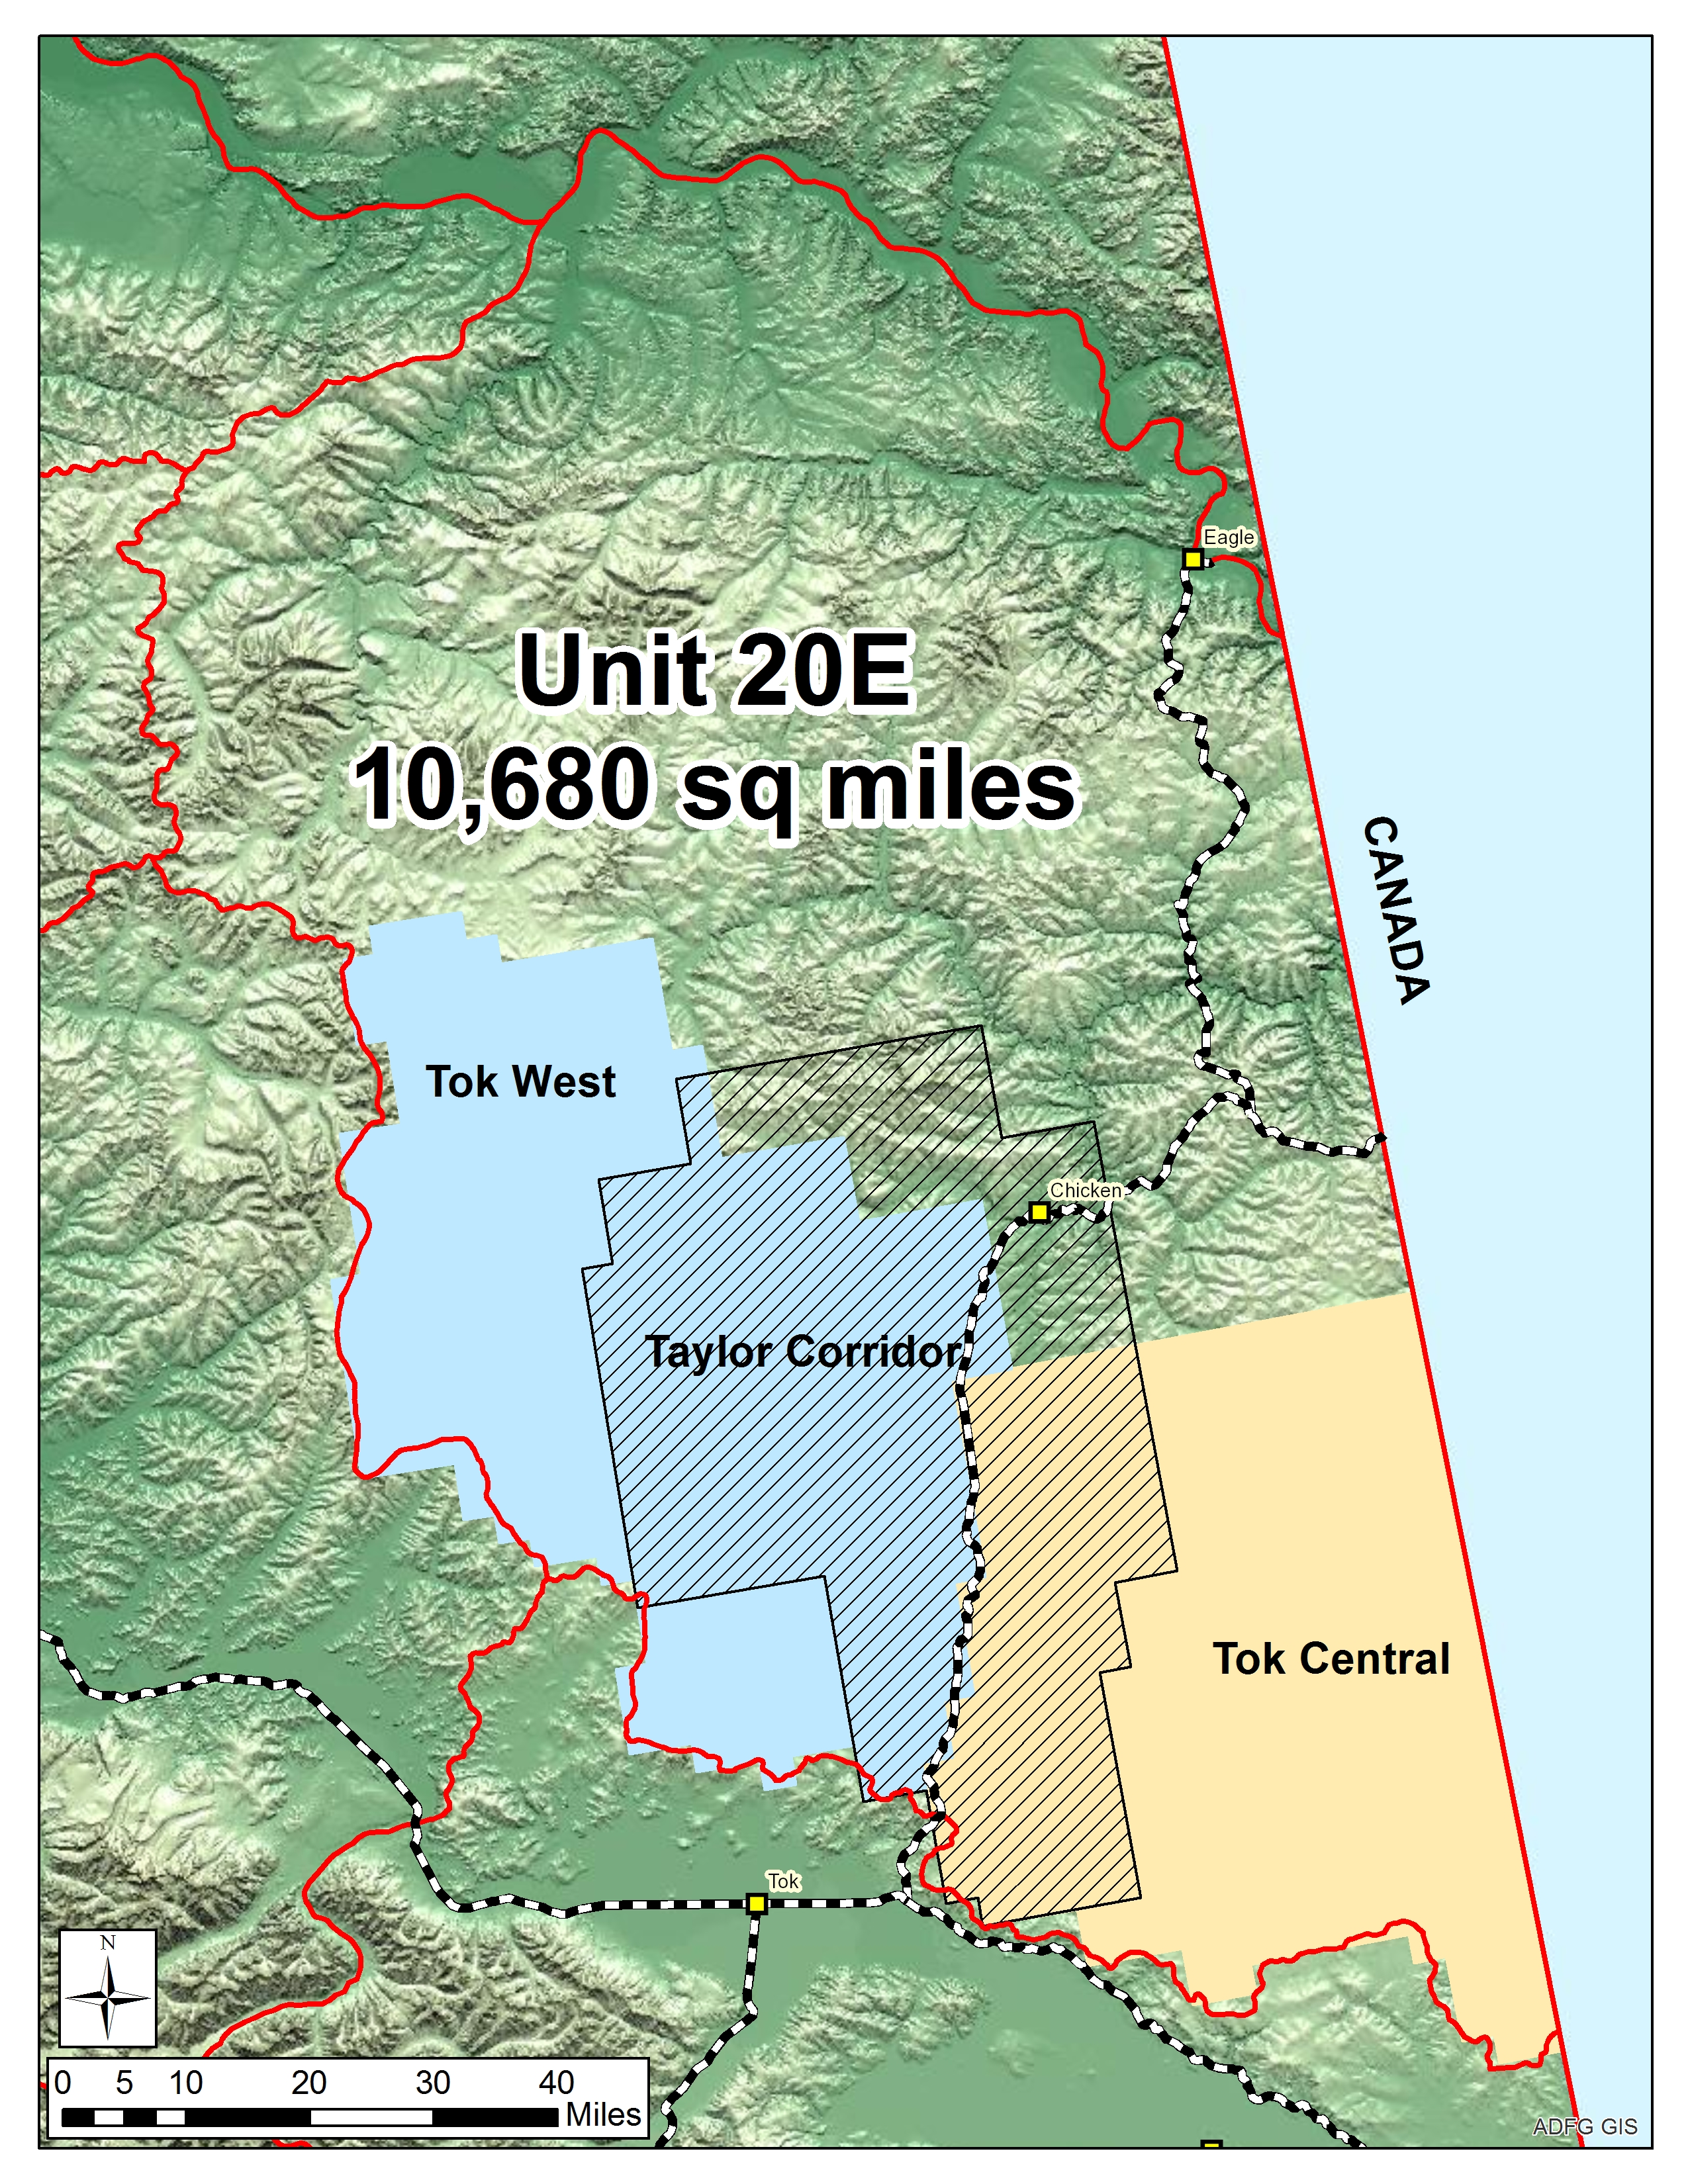
\includegraphics[width=0.5\linewidth]{20E_survey_area_overview} \caption{\label{fig:tokplot} A map of the Taylor Corridor in the TOK region of Alaska.}\label{fig:tokplot}
\end{figure}

Abundance surveys are performed in the Taylor Corridor of the TOK region
of Alaska annually (Figure \ref{fig:tokplot}). In particular, surveys
were conducted every year from 2014 through 2020, except for the year
2016, during which there was not sufficient snow cover to perform a
survey. There are a total of 381 unique spatial locations, which we
refer to as ``sites,'' and a total of 7 unique time points in the data
set, including the missing year of 2016.

In each year of the survey, an aerial team of biologists selects some of
the 381 sites to survey. The number of sites in the sampling frame that
are selected varies from a low of 76 in the year 2019 to a high of 90 in
the year 2020. Throughout the 7 unique time points, some sites are
surveyed as many as four or five different times while others are never
surveyed (Figure \ref{fig:tokplotyears}).

\begin{figure}
\centering
\includegraphics{fpspatiotemp_manu_files/figure-latex/tokplotyears-1.pdf}
\caption{\label{fig:tokplotyears} Layout of the spatial sites used to
survey moose in the Taylor corridor of the TOK region of Alaska.}
\end{figure}

Before the survey begins in each year, biologists stratify the sites
into a \texttt{"HIGH"} stratum and a \texttt{"LOW"} stratum. There are
230 sites in the \texttt{"HIGH"} stratum while there are 151 sites in
the \texttt{"LOW"} stratum. The goal of the following analysis is to
predict the total abundance of moose across all spatial sites in the
year \texttt{2020}, the most recent year of the survey.

\subsection{Model Fitting} \label{subsection:modelfit}

We fit the product-sum covariance model defined in equation
\ref{equation:model} using REML, with stratum as a covariate in the
design matrix, an exponential spatial correlation structure defined in
\ref{equation:spatcov}, and an exponential temporal correlation
structure defined in \ref{equation:tempcov}. Table \ref{paramest} gives
the estimated parameters from the model fit.

\begin{table}[ht]
\centering
\begin{tabular}{rrrrrrrrr}
  \hline
 & $\hat{\sigma}^2_{\delta}$ & $\hat{\phi}$ & $\hat{\sigma}^2_{\gamma}$ & $\hat{\sigma}^2_{\tau}$ & $\hat{\rho}$ & $\hat{\sigma}^2_{\eta}$ & $\hat{\sigma}^2_{\omega}$ & $\hat{\sigma}^2_{\nu}$ \\ 
  \hline
 & 16.9 & 4.44 & 3.8 & 0.9 & 2.29 & 0.2 & 30.8 & 24.0 \\ 
   \hline
\end{tabular}
\caption{Estimated covariance parameters in the model. $\hat{\sigma}^2_{\delta}$, $\hat{\sigma}^2_{\tau}$, and $\hat{\sigma}^2_{\eta}$ are the estimated spatial, temporal, and spatiotemporal partial sills, respectively, $\hat{\phi}$ and $\hat{\rho}$ are the estimated spatial and temporal range parameters, and $\hat{\sigma}^2_{\gamma}$, $\hat{\sigma}^2_{\omega}$, and $\hat{\sigma}^2_{\nu}$ are the estimated spatial, temporal, and spatiotemporal nuggets.} 
\label{paramest}
\end{table}

To help interpret what some of these fitted covariance parameter
estimates mean, we can construct a fitted covariance plot (Figure
\ref{fig:covplot}). Note that the centroids of two sites directly
adjacent to one another are about 4 units apart. As the spatial distance
between two sites increases (dark colour to light colour), the
covariance between the response values decreases to 0. In fact, the
model estimates the covariance to be nearly 0 when two sites are 20 or
more units apart, no matter what the temporal distance is. Note that the
fact that the covariance is larger than 0 when temporal distance is 6
and the spatial distance is either 0 implies that including surveys
before 2014 could improve precision of the predictor for the total
abundance in 2020 even more.

The estimated vector of fixed effects, using \texttt{"HIGH"} as the
reference group, is \(\bm{\beta}\) = (11.26, -9.76). Therefore the
overall mean for sites in the \texttt{"HIGH"} stratum is estimated to be
11.26 moose while the overall mean for sites in the \texttt{"LOW"}
stratum is estimated to be 1.5 moose.

\begin{figure}
\centering
\includegraphics{fpspatiotemp_manu_files/figure-latex/covplot-1.pdf}
\caption{\label{fig:covplot} Estimated covariance of the errors from the
fitted parameters in a product-sum model.}
\end{figure}

\subsection{Prediction}

We now use the model in subsection \ref{subsection:modelfit} to predict
the total abundance across all sites in the year 2020, the most recent
year of the survey. Plugging in estimates of the covariance parameters
into equations \ref{equation:lambdacurrentpred} and
\ref{equation:lambdacurrentvar} and letting elements of \(\mathbf{b}_a\)
be 1's for data points in 2020 and 0's otherwise, we obtain a prediction
of 2874 moose and a standard error of 234 moose. A 90\% normal-based
prediction interval for the total abundance in 2020 is (2489, 3259)
moose. Sitewise predictions for sites in 2020 are given in the map in
Figure \ref{fig:sitepredmap}.

\begin{figure}
\centering
\includegraphics{fpspatiotemp_manu_files/figure-latex/unnamed-chunk-8-1.pdf}
\caption{\label{fig:sitepredmap} A map of the predictions for the sites
in the year 2020. A site with a grey dot in the center means that the
site was sampled in 2020.}
\end{figure}

For comparison, we use the spatial \texttt{sptotal} package
\citep{higham2021sptotal} to compute the prediction for the total
abundance of moose in the year 2020 \citep{ver2008spatial}. We also use
the standard simple random sampling estimator \mbox{} \begin{equation*}
\bar{y} \cdot \frac{n_s}{n_{o}},
\end{equation*} \noindent where \(\bar{y}\) is the sample mean for the
data points in 2020, \(n_s\) is the total number of sites in 2020, and
\(n_o\) is the number of observed data points in 2020. The simple random
sampling estimator has a variance for the total abundance of
\(n_s^2 \cdot \frac{\hat{\sigma}^2}{n_o} \cdot (1 - \frac{n_o}{n_s})\).
Note that the purely spatial model fit with \texttt{sptotal} and the
simple random sampling estimator \textbf{only} use data from 2020.

For the purely spatial model, the prediction for the total number of
moose in 2020 in the region is 2870 moose with a standard error of 319
moose. For the simple random sampling estimator, the estimated total
number of moose in 2020 in the region is 3052 moose with a standard
error of 374 moose. While the predictions for the total are somewhat
similar across the three methods, we see that the spatiotemporal model
is most efficient (\(SE\) = 234 moose compared to 319 moose for the
purely spatial model and 374 moose for the simple random sampling
estimator that ignores both spatial and temporal information).

\section{Simulation} \label{section:Simulation}

\subsection{Description}

To evaluate performance of the finite population spatiotemporal model,
we conduct a small simulation study. We simulate a response vector
\(\mathbf{y}\) of length \(N = 1000\) on a \(10 \times 10\) grid of 100
spatial sites on the unit (\([0, 1] \times [0, 1]\)) square and 10
equally-spaced time points in the interval \([0, 1]\) (so that each
spatial site has a response value at each time point). \(\mathbf{y}\) is
multivariate normal with mean \(\mathbf{0}\) and product-sum covariance
matrix \(\bm{\Sigma}\) defined in equation \ref{equation:var} with the
covariance parameters given in Table \ref{tab:simparmtab}.

\begin{table}[H]

\caption{\label{tab:simparmtab}Covariance parameters used to simulate data. $\sigma^2_{\delta}$, $\sigma^2_{\gamma}$, and $\phi$ are the spatial dependent error variance, independent error variance, and range parameters, respectively. $\sigma^2_{\tau}$, $\sigma^2_{\eta}$, and $\rho$ are the temporal dependent error variance, independent error variance, and range parameters, respectively. $\sigma^2_{\omega}$ and $\sigma^2_{\nu}$ are the spatiotemporal dependent error variance and spatiotemporal independent error variance.}
\centering
\begin{tabular}[t]{ccccccccc}
\toprule
\multicolumn{1}{c}{ } & \multicolumn{3}{c}{Spatial} & \multicolumn{3}{c}{Temporal} & \multicolumn{2}{c}{Spatiotemporal} \\
\cmidrule(l{3pt}r{3pt}){2-4} \cmidrule(l{3pt}r{3pt}){5-7} \cmidrule(l{3pt}r{3pt}){8-9}
scenario & $\sigma^2_{\delta}$ & $\sigma^2_{\gamma}$ & $\phi$ & $\sigma^2_{\tau}$ & $\sigma^2_{\eta}$ & $\rho$ & $\sigma^2_{\omega}$ & $\sigma^2_{\nu}$\\
\midrule
spatiotemporal & 0.5 & 0.17 & 0.47 & 0.5 & 0.17 & 0.33 & 0.5 & 0.17\\
spatial & 0.0 & 0.00 & 0.47 & 0.0 & 0.00 & 0 & 1.5 & 0.50\\
independent & 0.0 & 0.00 & 0 & 0.0 & 0.00 & 0 & 0.0 & 2.00\\
\bottomrule
\end{tabular}
\end{table}

The three scenarios in the table correspond to (1)
\textbf{spatiotemporal}: a setting where there is spatiotemporal
covariance in the random errors, (2) \textbf{spatial}: a setting where
there is spatial covariance within a particular time point but errors in
different time points are not correlated even when the errors come from
the same spatial site, and (3) \textbf{independent}: all errors are
independent regardless of spatial index and time index. In all
scenarios, the total variance (summing all six variance parameters) is
equal to 2.

Both \(\mathbf{R}_{s}\) and \(\mathbf{R}_t\) are generated from the
exponential correlation function with \(\phi\) and \(\rho\) as the range
parameters in equations \ref{equation:spatcov} and
\ref{equation:tempcov}. The values \(0.471\) and \(0.3333\) are chosen
for \(\phi\) and \(\rho\), respectively, so that the effective ranges,
\(3 \phi\) and \(3 \rho\), are equal to the maximum distance between two
observations in space (\(\sqrt2 = 1.414\)) and the maximum distance
between two observations in time (\(1\)). A value of 0 for \(\phi\) (or
\(\rho\)) sets the \(\mathbf{R}_{s}\) matrix (or the \(\mathbf{R}_t\)
matrix) to the identity matrix.

Figure \ref{fig:simcovplot} shows the model covariance of the errors
used to generate data for the spatiotemporal scenario.

\begin{figure}
\centering
\includegraphics{fpspatiotemp_manu_files/figure-latex/unnamed-chunk-26-1.pdf}
\caption{\label{fig:simcovplot} The model covariance used in the
simulations for the spatiotemporal scenario. Covariance is approximately
0 for errors from observations that are \(\sqrt2\) distance units apart
in space and 1 distance unit apart in time. The spatial dependent error
variance (\(\sigma^2_{\delta}\)), spatial independent error variance
(\(\sigma^2_{\gamma}\)), temporal dependent error variance
(\(\sigma^2_{\tau}\)), and temporal independent error variance
(\(\sigma^2_{\eta}\)) are shown with grey lines.}
\end{figure}

Each of these three scenarios is replicated for two different sample
sizes: \(n = 250\) and \(n = 500\). A simple random sample of the 1000
total observations is used to select units to be in the sample.

Finally, the simulation experiment is repeated for a skewed response
variable. To create the skewed response variable, a normally-distributed
response is simulated according to the parameters given in Table
\ref{tab:simparmtab}, except that each of the variance parameters (not
including \(\phi\) and \(\rho\)) is divided by 2.89 so that the total
variance is equal to 0.6931. The resulting response variable is then
exponentiated so that the total variance after exponentiation is equal
to 2. Note that, not only does exponentiation result in a right-skewed
response variable, but exponentiating also allows for an assessment of
how the model performs when the covariance is misspecified, as the
resulting response variable no longer follows a tractable covariance
function.

Therefore, the simulation study has \(12\) total settings coming from a
\(3 \times 2 \times 2\) factorial design. For each setting, we simulate
1000 realizations. For each realization, we predict the total response
for the ``most recent'' time point (when the time index is equal to 1 on
the interval \([0, 1]\)), which we will henceforth call the ``current
total'' using three methods. The first method uses the finite population
kriging described in subsection \ref{subsection:fpbk} with the model
covariance in equation \ref{equation:var}. The second method is a
spatial model fit with the \texttt{sptotal} \texttt{R} package
\citep{higham2021sptotal} that only uses data from the most recent time
point. This method corresponds to how moose surveys are often currently
analyzed, assuming that abundance is correlated across space in the
survey but ignoring data from all previous surveys. Both of the first
two methods estimate model parameters with Restricted Maximum Likelihood
(REML). The third method uses a simple random sample (SRS) estimator
with data from the most recent time point. The SRS estimator for the
total is \(\bar{y} \cdot \frac{100}{n_1}\), where \(\bar{y}\) is the
sample mean of the response in the most recent time point and \(n_1\) is
the number of sampled locations in the most recent time point. The
variance is
\(n_1^2 \cdot \frac{\hat{\sigma}^2}{100} \cdot (1 - \frac{n_1}{100})\),
where \(\hat{\sigma}^2\) is the sample variance of the response variable
in the most recent time point.

Note that the SRS method gives an estimator (not a predictor) and
corresponding confidence interval (not a prediction interval) because
the estimator treats the observed data as fixed, not as a random
realization from a process
\citep{brus2021statistical, dumelle2022comparison}. However, in the
remaining text and tables, we refer to the ``current total'' response
quantity obtained from the three methods as a ``prediction'' and to the
corresponding interval as a ``prediction interval'' to limit
unnecessarily verbose text.

For each method, we record the root mean squared prediction error
(rMSPE), \(\sqrt{(\sum_{i = 1}^{1000}(\hat{T}_i - T_i)^2) / 1000}\),
where \(\hat{T}_i\) and \(T_i\) are the predicted and realized current
totals, respectively, in the \(i^{th}\) iteration. We also create a
normal-based 90\% prediction interval for the realized current total and
record both the average prediction interval length and the proportion of
iterations that the prediction interval covers the realized current
total.

\subsection{Results}

Tables \ref{tab:simrmspetab}, \ref{tab:simbiastab}, and
\ref{tab:simpitab} in Section \ref{section:appendix} give the rMSPE ,
bias and interval coverage of the three predictors in all 12 simulation
settings. In Figure \ref{fig:rmspe}, we see that the spatiotemporal
model outperforms both the purely spatial model and the simple random
sample design-based estimator in all 12 settings. In general, rMSPE is
improvement is larger for the smaller sample size. In general, as \(n\)
approaches \(N\), rMSPE for all approaches should become smaller and be
exactly equal to 0 when \(n = N\).

We also see that, in general, the smallest gains in rMSPE for the
spatiotemporal model are made in the ``spatial'' simulation setting. In
this setting, response values across space are only correlated within a
given time point; therefore, the spatiotemporal model only does
marginally better than the other two approaches because the data from
the other time points are not correlated with the data in the most
current time point. However, in both the independent setting and the
spatial setting, the spatiotemporal model still outperforms the purely
spatial model and the simple random sample design-based estimator
because the spatiotemporal can still use the response values collected
in previous time points to estimate the fixed effects structure of the
model.

\begin{figure}
\centering
\includegraphics{fpspatiotemp_manu_files/figure-latex/unnamed-chunk-28-1.pdf}
\caption{\label{fig:rmspe} root Mean-Squared-Prediction-Error for all
simulation settings. The spatiotemporal model has the smallest rMSPE in
all settings tested, though it is similar to the rMSPE of the other two
methods in the spatial scenario, where response values within a time
point are correlated across space but are uncorrelated with all response
values from other time points.}
\end{figure}

All methods appear relatively unbiased in all simulation settings: Table
\ref{tab:simbiastab} shows that the bias of each method is small
compared to the squares of the rMSPE values given in
\ref{tab:simrmspetab}.

Figure \ref{fig:pi} shows the interval coverage for the normal-based
prediction intervals, where the nominal level is 0.90. We see that the
spatiotemporal model predictor for the current total has approximate
90\% coverage in all settings tested. The spatial model and the SRS
design-based estimator have lower than nominal coverage in some settings
because of the small sample size used (recall that the \(n = 250\)
observed samples span 10 unique time points so that, on average, the
spatial model and SRS design-based estimator only have 25 observed
responses in the current time point).

\begin{figure}
\centering
\includegraphics{fpspatiotemp_manu_files/figure-latex/unnamed-chunk-29-1.pdf}
\caption{\label{fig:pi} Prediction interval coverage for all simulation
settings, where the prediction intervals are normal-based and the
nominal level is 0.90. The predictor from the spatiotemporal model has
close to appropriate coverage in all settings tested.}
\end{figure}

\section{Discussion} \label{section:Discussion}

\begin{itemize}
\item
  substantial reduction of se in the application (and, presumably, the
  simulations).

  \begin{itemize}
  \tightlist
  \item
    if there is a very high amount of spatial correlation but a low
    amount of temporal correlation (as in the second scenario), then
    gains are minimal.
  \end{itemize}
\item
  normal-based-related limitations
\item
  Bayesian approach, and its drawbacks benefits to bayes: - models
  counts as counts (better for predicting on one particular site) -
  model more expandable (lots of zeroes eg.) benefits to ours: - much
  quicker - assessed via a small simulation study - easier for
  practitioner to fit (especially given software - no convergence
  checks, priors to be tweaked, etc.)
\end{itemize}

An additional possible benefit of the spatiotemporal model compated to a
purely spatial model is the potential for forecasting abundance before a
survey is done. For example, in our application, we can refit the model
without any of the observed counts from the 2020 survey and examine the
prediction for the total abundance in 2020. Table \ref{tab:forecast}
compares the model with the 2020 data used and the model without the
2020 data used. We see that, while there is a substantial loss in
precision by excluding the 2020 data (as we would expect), the
prediction is not very different from the prediction with the 2020 data
included and the prediction interval might be narrow enough to still be
useful to biologists. We might also consider using such an approach if
there is a year during which a survey cannot be completed for logistical
reasons. For example, in the TOC region of Alaska, a moose survey was
not conducted at all in the year 2016 because there was insufficient
snow cover for the survey. The spatiotemporal could still be applied to
get a prediction for moose abundance using survey data from previous
years.

\begin{table}[H]

\caption{\label{tab:forecast}Results from analysis on the TOC moose survey data with the 2020 survey included and excluded. We can see that, even with 2020 data excluded, we can obtain a prediction for moose abundance in 2020, though there is substantial loss in precision.}
\centering
\begin{tabular}[t]{lcccc}
\toprule
  & Prediction & SE & 90\% LB & 90\% UB\\
\midrule
2020 Data Included & 2874 & 234 & 2489 & 3259\\
2020 Data Excluded & 2757 & 417 & 2071 & 3444\\
\bottomrule
\end{tabular}
\end{table}

There is a substantial drop in efficiency when 2020 is not surveyed, but
some monitoring programs may deem this worthy, or, might find this
useful if a survey cannot be done one year because of poor conditions,
changes in personnel, etc. (and it might drop more or not as much
depending how the temporal correlation structure).

\begin{itemize}
\tightlist
\item
  take-home message: monitoring programs that use regularly-scheduled
  surveys might consider incorporating time into their analysis to
  improve precision of predictors for the mean or total.
\end{itemize}

\section{Appendix} \label{section:appendix}

\begin{table}[H]

\caption{\label{tab:simrmspetab}root Mean Squared Prediction Error (rMSPE) for the spatiotemporal model, the spatial model, and the simple random sample estimator for each of the 12 simulation settings. In all settings, the rMSPE for the spatiotemporal model is lower than the rMSPE for the other two methods.}
\centering
\begin{tabular}[t]{cccccc}
\toprule
\multicolumn{3}{c}{Simulation Setting} & \multicolumn{3}{c}{rMSPE} \\
\cmidrule(l{3pt}r{3pt}){1-3} \cmidrule(l{3pt}r{3pt}){4-6}
scenario & n & Response Type & spatiotemporal & spatial & srs\\
\midrule
independent & 250 & normal & 14.81 & 25.36 & 24.82\\
spatial & 250 & normal & 18.62 & 19.30 & 21.35\\
spatiotemporal & 250 & normal & 11.89 & 15.56 & 17.30\\
\midrule
independent & 500 & normal & 10.89 & 14.44 & 14.33\\
spatial & 500 & normal & 10.17 & 10.30 & 12.43\\
spatiotemporal & 500 & normal & 6.08 & 8.35 & 9.92\\
\midrule
independent & 250 & lognormal & 15.39 & 27.21 & 25.61\\
spatial & 250 & lognormal & 20.41 & 21.13 & 22.16\\
spatiotemporal & 250 & lognormal & 15.32 & 17.24 & 19.41\\
\midrule
independent & 500 & lognormal & 10.93 & 14.45 & 14.33\\
spatial & 500 & lognormal & 10.93 & 11.19 & 12.65\\
spatiotemporal & 500 & lognormal & 7.99 & 9.25 & 11.08\\
\bottomrule
\end{tabular}
\end{table}

\begin{table}[H]

\caption{\label{tab:simbiastab}Bias (Realized Current Total - Predicted Current Total) for the spatiotemporal model, the spatial model, and the simple random sample estimator for each of the 12 simulation settings. In all settings, all methods appear fairly unbiased.}
\centering
\begin{tabular}[t]{cccccc}
\toprule
\multicolumn{3}{c}{Simulation Setting} & \multicolumn{3}{c}{Bias} \\
\cmidrule(l{3pt}r{3pt}){1-3} \cmidrule(l{3pt}r{3pt}){4-6}
scenario & n & Response Type & spatiotemporal & spatial & srs\\
\midrule
independent & 250 & normal & -0.16 & -0.30 & -0.37\\
spatial & 250 & normal & -0.44 & -0.37 & -0.69\\
spatiotemporal & 250 & normal & -0.01 & 0.17 & -0.63\\
\midrule
independent & 500 & normal & 0.01 & 0.05 & 0.00\\
spatial & 500 & normal & -0.10 & -0.10 & -0.29\\
spatiotemporal & 500 & normal & -0.05 & 0.02 & -0.47\\
\midrule
independent & 250 & lognormal & -0.17 & -1.20 & -0.37\\
spatial & 250 & lognormal & -0.73 & -1.11 & -0.65\\
spatiotemporal & 250 & lognormal & -0.06 & 0.15 & -0.24\\
\midrule
independent & 500 & lognormal & 0.35 & 0.18 & 0.31\\
spatial & 500 & lognormal & -0.23 & -0.47 & -0.46\\
spatiotemporal & 500 & lognormal & 0.00 & -0.12 & -0.61\\
\bottomrule
\end{tabular}
\end{table}

\begin{table}[H]

\caption{\label{tab:simpitab}Prediction interval coverage for the spatiotemporal model, the spatial model, and the simple random sample estimator for each of the 12 simulation settings. All intervals are normal-based and have a nominal coverage level of 0.90.}
\centering
\begin{tabular}[t]{cccccc}
\toprule
\multicolumn{3}{c}{Simulation Setting} & \multicolumn{3}{c}{Coverage} \\
\cmidrule(l{3pt}r{3pt}){1-3} \cmidrule(l{3pt}r{3pt}){4-6}
scenario & n & Response Type & spatiotemporal & spatial & srs\\
\midrule
independent & 250 & normal & 0.92 & 0.88 & 0.89\\
spatial & 250 & normal & 0.89 & 0.86 & 0.89\\
spatiotemporal & 250 & normal & 0.88 & 0.87 & 0.90\\
\midrule
independent & 500 & normal & 0.90 & 0.89 & 0.89\\
spatial & 500 & normal & 0.89 & 0.88 & 0.90\\
spatiotemporal & 500 & normal & 0.89 & 0.87 & 0.89\\
\midrule
independent & 250 & lognormal & 0.91 & 0.84 & 0.85\\
spatial & 250 & lognormal & 0.88 & 0.83 & 0.87\\
spatiotemporal & 250 & lognormal & 0.87 & 0.85 & 0.87\\
\midrule
independent & 500 & lognormal & 0.90 & 0.88 & 0.88\\
spatial & 500 & lognormal & 0.89 & 0.87 & 0.88\\
spatiotemporal & 500 & lognormal & 0.89 & 0.87 & 0.89\\
\bottomrule
\end{tabular}
\end{table}

\bibliographystyle{tfcad}
\bibliography{interactcadsample.bib}





\end{document}
